% !TeX root = ../../main.tex
\subsection{大容量强磁吸附工具结构及工作原理}
\label{darongliangqiangci}
大容量强磁吸附工具用于打捞套管修复或清洁作业过程中产生的不能被循环液返出的磁性碎物，通过永久磁铁吸附磁性碎物将其带出井筒，实现井筒净化效果。针对不同尺寸磁性碎物，磁铁套筒有两种吸附模式，一种是沿侧面沟槽方向吸附（以下简称“侧吸”），另一种是沿圆周方向吸附（以下简称“环吸”），两种强磁均具有保护层，可单独更换强磁块，且强磁块固定未采用螺钉连接，方便装卸且结构稳定。针对套管中磁性碎物的含量，可以预先装配不同数量的磁铁套筒，以匹配强磁吸附工具容量和磁性碎物量。该工具具有结构可靠、操作方便、多方向，多尺寸吸附、碎屑吸附量大和可调节等优点。

强磁工具主要由上接头、上连接套、侧吸强磁部件、中间连接套、环吸强磁部件、止退环、下接头等零件组成。
通过永久磁铁吸附磁性碎物并将其带出井筒，从井下回收不能被循环液返出的磁性碎物，从而实现井筒净化效果。


\begin{table}[htbp]
    \centering
    \caption{强磁工具技术参数}
    \label{tab:dqc_parameters}
    \renewcommand{\arraystretch}{1.3} % 增加行高，使表格不拥挤
    \small % 如果表格太宽，可以使用 \small 或 \footnotesize 微调字号
    
    % 使用 tabularx 环境，总宽度设为 \textwidth
    % 列定义说明：
    % l: 左对齐（型号）
    % c: 居中对齐（数值类数据）
    % X: 自动伸缩列（用于较长文本或为了撑满宽度的列，这里用于平衡布局）
    \begin{tabularx}{.9\textwidth}{l ccc Xc ccc c} 
        \toprule
        % 表头内容
        规格 & 
        \begin{tabular}[c]{@{}c@{}}接头\\外径\\ (mm)\end{tabular} & 
        \begin{tabular}[c]{@{}c@{}}扶正\\外径\\ (mm)\end{tabular} & 
        \begin{tabular}[c]{@{}c@{}}本体\\外径\\ (mm)\end{tabular} & 
        \begin{tabular}[c]{@{}c@{}}适用套\\管磅级\\ (lb/ft)\end{tabular} & 
        \begin{tabular}[c]{@{}c@{}}水眼\\ (mm)\end{tabular} & 
        \begin{tabular}[c]{@{}c@{}}总长\\ (mm)\end{tabular} & 
        \begin{tabular}[c]{@{}c@{}}接头\\螺纹\\ (API)\end{tabular} & 
        \begin{tabular}[c]{@{}c@{}}抗拉\\强度\\ (T)\end{tabular} & 
        \begin{tabular}[c]{@{}c@{}}抗扭\\强度\\ (kN$\cdot$m)\end{tabular} \\
        \midrule
        
        % 数据行
        7\inch  & 127    & 141.5  & 139.7  & 9.5-40.5 & 40    & 6500 & NC38      & 180 & 21  \\
        9-5/8\inch  & 165    & 185.93 & 184.15 & ALL      & 57.15 & 6500 & NC50      & 350 & 30  \\
        13-3/8\inch  & 196    & 236.73 & 234.95 & ALL      & 76.2  & 6500 & 6 5/8 REG & 500 & 60  \\
        
        \bottomrule
    \end{tabularx}
\end{table}
%[c]{@{}c@{}}中方括号内的 [c] 是垂直对齐参数，用于控制该 tabular 环境作为一个整体在其所在行中的垂直位置。@{}c@{} 是表格列格式定义，其核心作用是控制单元格内容的对齐方式并消除列间默认间距，常用于嵌套表格或需要精确对齐的场景
%lb/ft为“磅每英尺”，lb 是英制质量单位磅（Pound）的缩写，英语中的 "pound" 一词本身就源自拉丁语 pondus（重量），因此保留了 libra 的缩写 lb 作为符号

\subsection{强磁工具结构设计}

强磁工具采用长轴式结构，沿轴向由上接头、上连接套、侧吸强磁部件、中间连接套、环吸强磁部件、止退环和下接头依次连接而成，如图\ref{fig:structure_dqc_mag_tool}所示。工具中心设有贯通的循环水眼，水眼直径分别为40、57.15和76.2mm，保证工具在下放、循环和起出过程中不影响井筒正常循环；工具外圆设有扶正结构，扶正外径分别为141.5、185.93和236.73mm，使强磁部件在套管内保持居中，避免强磁部件与套管内壁直接碰撞。工具总长为6500mm，上、下接头螺纹分别为NC38、NC50和6\,5/8\,REG，依次适用于7\inch、9-5/8\inch 和13-3/8\inch 套管，相应形成DQC700000A、DQC962500A和DQC133800A三个型号。

\begin{figure}[htbp]
    \centering
    % 子图 (a)
    \subfloat[工具总体结构]{%
        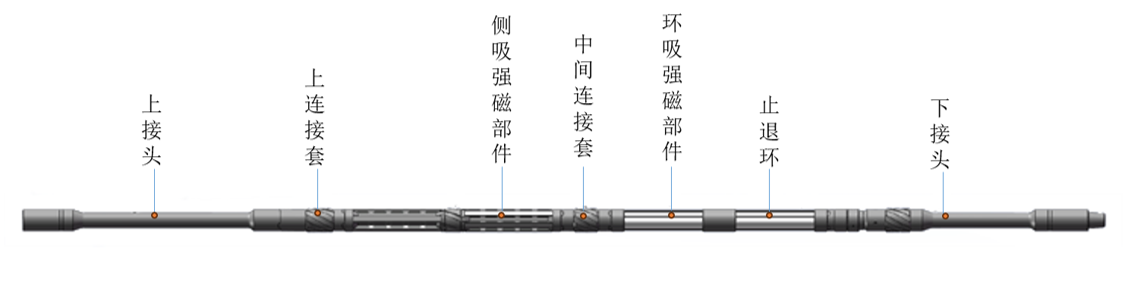
\includegraphics[width=0.9\linewidth]{figure/chapter3/structure-dqc-mag-tool.png}%
        \label{fig:structure_dqc_mag_tool}%
    }
    \vspace{1em}
    % 子图 (b)
    \subfloat[侧吸强磁局部结构]{%
        \includegraphics[width=0.4\linewidth]{figure/chapter3/structure-upper-magnetic-sub.png}%
        \label{fig:magnetic_tool_upper_sub}
    }
    \hfill
    % 子图 (c)
    \subfloat[环吸强磁局部结构]{%
        \includegraphics[width=0.4\linewidth]{figure/chapter3/structure-lowwer-magnetic-sub.png}%
        \label{fig:magnetic_tool_lowwer_sub}%
    }
        \caption{大容量强磁工具含磁结构示意图}
    \label{fig:structure_magnetic_tool}
\end{figure}

侧吸强磁部件（对应工具侧吸强磁结构）用于吸附小尺度磁性碎屑，主要由带窗强磁保护管、导磁骨架和永磁块组成，其局部结构见图\ref{fig:structure_magnetic_tool}(b)。永磁块安装于保护管内部，保护管沿周向开窗，使永磁体表面能够与井筒内的磁性碎屑直接接触，增大有效吸附面积；骨架沿轴向加工出吸附沟槽，碎屑主要积存于相邻吸附单元之间的沟槽中，每个吸附单元包含两组永磁块。工具上端设有两个强磁架，两者结构相同，单个强磁架上沿轴向布置5条吸附沟槽。

环吸强磁部件（对应工具环吸强磁结构）用于吸附大尺度磁性碎屑，其局部结构见图\ref{fig:structure_magnetic_tool}(c)。永磁块沿骨架圆周方向均匀布置，其外圆面面积大，使大尺寸铁屑能够直接吸附于永磁体表面。工具下端同样设有两个强磁架，两者结构相同。

两种强磁部件均设有保护层：侧吸强磁的永磁块安装于带窗的不锈钢保护管内，环吸强磁的永磁块安装于开放式骨架内，保护层可将运输、装配与下井过程中产生的机械冲击以及井筒内的腐蚀性介质与磁材本体隔离开来，磁块在制造时表面还采用镀镍处理。永磁块的固定不采用螺钉连接，各永磁块均可单独拆卸、更换，既便于工具的装配与现场维护，也避免了井下振动引起螺钉松脱的问题。

工具各功能单元之间通过螺纹与心轴连接，心轴的连接螺纹为2.85\inch-8 Stub ACME（图纸DQC700003A--心轴，标准ASME B1.8）。为防止扭矩与振动作用下螺纹退扣，连接部位设有止退环，并由下接头端面键承担主要防退扣扭矩，下接头端面上设有6个端面键（图纸DQC700007A--下接头），键宽$b$与键高$h$按图纸端面键截面实测，取$b=19\,\text{mm}$、$h=11.75\,\text{mm}$，端面键截面为防退扣结构的薄弱环节。各危险截面的螺纹剪切、抗拉、抗扭及防退扣强度校核见\ref{sec:mag_tool_check}节。

针对套管中磁性碎物的含量，可通过预先装配不同数量的磁铁套筒匹配工具的吸附容量与碎屑量，从而实现吸附容量的调节。以7\inch、17lb/ft套管（壁厚5.87mm、内径166.06mm）为例，单根工具的吸附容量为28.26L，两根工具组合后的吸附容量为56.52L，可满足吸附容量不小于50L的设计要求，具体计算见\ref{sec:mag_tool_check}节。

强磁工具的主要受力件为心轴，其材料为4330V-155KSI，最小屈服强度为930MPa；强磁骨架选用4145钢，永磁体保护套选用304不锈钢，永磁体选用耐温性与抗退磁能力更好的钐钴（SmCo5）材料。骨架作为工具磁路的一部分，宜选用导磁效果好、可磁化程度高的金属材料，以起到聚集磁感线、增大磁通的作用；永磁体的充磁方式及其对工具表面磁场分布的影响见后文磁铁布置研究。

强磁工具的主要结构参数汇总于表\ref{tab:mag_tool_structure_params}中。由上述结构设计可知，强磁工具通过侧吸强磁部件与环吸强磁部件的组合，实现了沿沟槽方向和沿圆周方向的多方向、多尺寸磁性碎屑吸附；永磁块可单独更换、装配数量可根据碎物含量调节，工具具有结构可靠·、装卸方便、吸附容量大且可调节等优点。

\begin{table}[htbp]
    \centering
    \caption{强磁工具主要结构参数}
    \label{tab:mag_tool_structure_params}
    \renewcommand{\arraystretch}{1.3} % 增加行高，使表格不拥挤
    \begin{tabularx}{.9\textwidth}{CCCC}
        \toprule
        构件 & 结构参数 & 符号 & 数值 \\
        \midrule
        强磁部件 & 强磁架数量 & -- & 4个（上端2个、下端2个，同端两强磁架结构相同） \\
        \midrule
        \multirow{5}{*}{侧吸强磁部件} & 沟槽数量（单个强磁架） & -- & 5条 \\
         & 沟槽截面面积 & $s$ & $603\,\text{mm}^2$ \\
         & 吸附沟槽长度 & $h$ & $500\,\text{mm}$ \\
         & 环空面积 & $s_1$ & $7340\,\text{mm}^2$ \\
         & 环空长度 & $h_1$ & $1438\,\text{mm}$ \\
        \midrule
        \multirow{2}{*}{环吸强磁部件} & 环空面积 & $s_2$ & $10343\,\text{mm}^2$ \\
         & 环空长度 & $h_2$ & $1420\,\text{mm}$ \\
        \midrule
        下接头 & 端面键 & -- & 6个（材料4145H，$b=19\,\text{mm}$，$h=11.75\,\text{mm}$） \\
        \bottomrule
    \end{tabularx}
\end{table}

%注：表中$s$、$s_1$、$s_2$、$h$、$h_1$、$h_2$为强磁工具吸附容量计算所采用的结构参数，均由强磁架零件图及DQC700000A总装图实测得到，其定义及取值来源见\ref{sec:mag_tool_check}节。

\subsubsection{与国外同类强磁工具的对比分析}
\label{sec:mag_tool_compare}

目前国外具有代表性的井筒磁性碎屑打捞工具为 Schlumberger／M-I SWACO 公司的 MAGNOGARD 裸眼强磁工具。该工具安装于钻头上方，主要用于裸眼钻井期间吸附井筒内的铁磁性碎屑，以延长钻头寿命、降低下部钻具组合的损伤，并使下入完井管柱前的裸眼井段不含钢质碎屑；据其公开产品样本，该工具额定耐温 $204\,^\circ\mathrm{C}$，采用整体式高强度心轴、无内部连接，外圆为流线型设计，可在裸眼井段中旋转与往复运动而不损伤工具与地层，本体设有耐磨磨光的碳化钨区域，磁体沿圆周方向布置，并设大容量收集槽，使吸附的铁屑在起出地面之前保持在槽内而不落回井筒。两者同属井筒磁性碎屑的井下打捞工具，但本工具面向完井、修井以及磨铣、射孔后的套管内井筒清洁作业，主要技术特点对比见表~\ref{tab:mag_tool_compare}\footnote{表中 MAGNOGARD 工具的相关数据引自其公开产品样本，仅用于技术特点的对比说明。}。

\begin{table}[htbp]
    \centering
    \caption{本强磁工具与 MAGNOGARD 裸眼强磁工具的技术特点对比}
    \label{tab:mag_tool_compare}
    \footnotesize
    \setlength{\tabcolsep}{4pt}
    \renewcommand{\arraystretch}{1.3}
    \begin{tabularx}{\textwidth}{lCC}
        \toprule
        对比项目 & MAGNOGARD 裸眼强磁工具 & 本大容量强磁吸附工具 \\
        \midrule
        适用工况与定位 & 裸眼钻井期间随钻打捞，安装于钻头上方，用于保护钻头与下部钻具组合 & 完井、修井及磨铣、射孔后套管内井筒清洁，随工具串下入，打捞不能被循环液返出的磁性碎屑 \\
        \midrule
        磁体布置方式 & 磁体沿圆周方向布置，设大容量收集槽 & 上部侧吸部件沿侧面沟槽定向吸附，下部环吸部件沿圆周全角度吸附，两个吸附单元沿轴向分区协同 \\
        \midrule
        吸附能力指标 & 样本未给出吸附力与表面磁感应强度的量化指标 & 吸附力 $\ge 8\,\text{kg/cm}^2$、磁铁表面磁感应强度 $\ge 1.42\,\text{T}$，可逐支检验 \\
        \midrule
        吸附容量 & 样本以“大容量收集槽”定性描述 & 7\inch 规格单根工具 $28.26\,\text{L}$、两根工具串接 $56.52\,\text{L}$，按结构参数计算并可验收 \\
        \midrule
        磁块固定与更换 & 样本未说明 & 磁块免螺钉固定、定位可靠，可单块更换，装配数量可按碎屑含量调整 \\
        \midrule
        耐温指标 & 额定 $204\,^\circ\mathrm{C}$ & 按合同 $\ge 150\,^\circ\mathrm{C}$ 设计，选用烧结钐钴 SmCo5，最高工作温度 $250\sim 350\,^\circ\mathrm{C}$，$150\,^\circ\mathrm{C}$ 保温 $2\,\text{h}$ 后不可逆磁通损失 $<5\%$ \\
        \midrule
        结构形式与流道 & 整体式高强度心轴，无内部连接，流线型外圆，本体设耐磨碳化钨区域 & 长轴式结构，中心为贯通水眼（$\phi$40、$\phi$57.15、$\phi$76.2\,mm），外圆设扶正结构（扶正外径 $141.5$、$185.93$、$236.73\,\text{mm}$） \\
        \midrule
        强度设计校核 & 样本未给出 & 心轴 2.85\inch-8 Stub ACME 螺纹牙剪切 $2951.7\,\text{kN}$，内、外螺纹根部许用拉力 $1627.42$、$2462.93\,\text{kN}$，许用扭矩 $35.98$、$86.29\,\text{kN}\cdot\text{m}$，下接头端面键按 6 键同时受剪计算的许用防退扣扭矩 $35.7\,\text{kN}\cdot\text{m}$ \\
        \bottomrule
    \end{tabularx}
\end{table}



\begin{figure}[htbp]
    \centering
    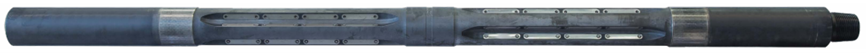
\includegraphics[width=0.95\textwidth]{figure/chapter3/magnogard-magnet-tool.png}
    \caption{MAGNOGARD 裸眼强磁工具外形（图片来源：公开产品样本）}
    \label{fig:magnogard_tool}
\end{figure}

与上述参照工具相比，本工具的设计优势主要体现在以下几个方面。

（1）吸附单元分区布置，不同尺度碎屑兼收。本工具上部侧吸部件沿侧面沟槽定向吸附，适用于吸附毫米级铁质颗粒；下部环吸部件为开放式结构，环空面积 $10343\,\text{mm}^2$、环空长度 $1420\,\text{mm}$，适用于吸附尺度较大的铁质碎屑。两类吸附单元沿轴向分区布置，可在同一趟钻内完成不同尺度磁性碎屑的收集；与仅沿圆周方向布置磁体的结构形式相比，其吸附方向与适用碎屑尺度更为明确。

（2）吸附能力以可检验的量化指标控制。本工具的吸附能力以吸附力与磁铁表面磁感应强度两项指标控制，要求对 45 钢铁屑的吸附力 $\ge 8\,\text{kg/cm}^2$，对应磁铁表面磁感应强度 $\ge 1.42\,\text{T}$，两项指标均可在出厂前逐支检验；吸附容量则按强磁架零件图及总装图实测的结构参数计算，7\inch 规格单根工具为 $28.26\,\text{L}$、两根工具串接为 $56.52\,\text{L}$，大于合同规定的 $50\,\text{L}$。参照工具的样本资料仅以“大容量收集槽”作定性描述，未给出可供检验的吸附能力指标。

（3）磁块免螺钉固定，杜绝磁块遗留井内。本工具的强磁块采用免螺钉安装结构，装配后由磁铁保护管与卡环定位，定位可靠且便于单块拆装，可根据套管内径与碎屑情况调整装配数量；由于井下不存在螺钉松脱的环节，避免了磁块脱落遗留井内的风险。参照工具样本未说明其磁块的固定与更换方式。

（4）磁路设计具备完整的选型与仿真依据。本工具依据合同 $\ge 150\,^\circ\mathrm{C}$ 的耐温指标，对比钐钴（SmCo5）与钕铁硼（N45UH）等永磁材料的退磁曲线后确定选用烧结钐钴材料；通过骨架材料的对比仿真确定采用导磁效果好的 4145 钢骨架，相较铝制骨架，永磁体表面磁感应强度由 $0.3\sim 0.7\,\text{T}$ 提高至 $0.7\sim 1.5\,\text{T}$、骨架沟槽表面由 $0.2\sim 0.4\,\text{T}$ 提高至 $1.2\sim 3.5\,\text{T}$；并基于 ANSYS Maxwell 对上、下部结构的充磁方式与磁场分布进行仿真优化，给出了优选的布置方案。

（5）主要受力件强度校核完整，覆盖螺纹连接与防退扣结构。本工具对心轴 2.85\inch-8 Stub ACME 螺纹的牙剪切强度、内螺纹与外螺纹根部拉伸强度、抗扭强度以及下接头端面键的防退扣能力均进行了计算与有限元复核，可满足抗拉 $100\,\text{T}$、抗扭 $18\,\text{kN}\cdot\text{m}$ 的设计指标；参照工具样本未给出相应的强度设计数据。

需要说明的是，参照工具样本给出的额定耐温为 $204\,^\circ\mathrm{C}$，高于本项目合同规定的 $150\,^\circ\mathrm{C}$ 耐温指标。本工具按合同指标设计，所选烧结钐钴 SmCo5 的最高工作温度为 $250\sim 350\,^\circ\mathrm{C}$，相对合同指标仍有 $100\,^\circ\mathrm{C}$ 以上的温度裕量，工具工作温度范围内发生的退磁均可逆，具备向更高温度井况拓展的余量。

\subsection[强磁工具结构设计计算与校核]{强磁工具结构设计计算与校核\protect\footnote{合同条款：5.2.1.3井筒高效清洁关键技术配套工具设计——（2）大容量强磁吸附工具：抗拉$>=100\mathrm{T}$，抗扭$>=18 \mathrm{kN}\cdot \mathrm{m}$，吸附力$>=8\mathrm{kg/cm^2}$，吸附容量$>=50\mathrm{L}$}}\label{sec:mag_tool_check}

%这里的强度校核与四合一工具的相同，我这里姑且写上，后面可以引用前面的内容并把这个注释掉。

大容量强磁工具的主要受力件为心轴，其连接螺纹为 2.85\inch-8 Stub ACME。螺纹牙剪切强度计算：

\begin{equation}
    \begin{aligned}
        F_{\max} &= [\tau] \cdot k_z \cdot \pi \cdot d_1 \cdot b \cdot z \times 10^{-3} \\
        [\tau] &= \frac{\sigma_{\mathrm{s}}}{n}
    \end{aligned}
\end{equation}
式中，$F_{\max}$--工具最大拉力，kN（设计指标 $\ge 1000$\,kN，见本节脚注所列合同条款 5.2.1.3（2）：抗拉 $\ge 100$\,T）；

$[\tau]$--螺纹牙的剪切强度，MPa（按 $[\tau]=\sigma_{\mathrm{s}}/n$ 计算）；

$k_z$--螺纹各圈的载荷不均系数，取 $k_z = 0.56$（按《机械设计手册》螺纹连接（紧固件连接）部分中螺纹牙的剪切强度计算及各圈螺纹载荷分配的规定\cite{ref26}）；

$d_1$--螺纹底径，取 70.30\,mm（图号 DQC700003A--心轴主视图标注的 2.85$''$-8 Stub ACME 外螺纹小径 70.485$\sim$70.643\,mm，偏安全取小值侧）；

$b$--螺纹牙根宽度，取 $b = 1.833\,\text{mm}$（按 ASME B1.8 规定的 ACME 牙型，由螺距 $p=25.4/8=3.175\,\text{mm}$ 与基本牙型高度 $h_0=p/2=1.588\,\text{mm}$ 计算）；

$n$--安全系数，取 $n = 2.5$（按《机械设计手册》螺纹连接部分中螺纹牙强度校核的安全系数取值规定\cite{ref26}）；

$z$--旋合圈数，取 $z = 35$（图号 DQC700003A--心轴外螺纹与配套内螺纹的旋合长度标注除以螺距 3.175\,mm 折合，偏安全取值）；

$\sigma_{\mathrm{s}}$--材料最小屈服强度，取 930\,MPa（图号 DQC700003A--心轴\ 技术要求：材料 4330V-155KSI，调质后屈服强度 $\ge 930$\,MPa）。


2.85\inch-8 Stub ACME 螺纹代入数据计算如下：
\begin{equation}
    \begin{aligned}
        F_{\max} &= [\tau] \cdot k_z \cdot \pi \cdot d_1 \cdot b \cdot z \times 10^{-3} \\
                &= 372 \times 0.56 \times 3.14 \times 70.30 \times 1.833 \times 35 \times 10^{-3} \\
                &= 2950.16 \, \text{kN} > 1000 \, \text{kN}
    \end{aligned}
\end{equation}
于是，螺纹的强度满足设计要求。

大容量强磁工具的主要受力件为心轴,危险截面有两处，分别为2.85\inch -8 Stub ACME外螺纹根部、2.85\inch-8 Stub ACME内螺纹根部。下面为心轴抗拉计算。
%这里的2.85是不是写错了

（1）轴抗拉危险截面1：2.85\inch -8 Stub ACME外螺纹根部

抗拉强度$F_{\max}$为
\begin{equation}
    \begin{aligned}
        F_{\max} &= \left[\pi \cdot (D^2 - d^2)\right] \cdot \sigma_{\mathrm{s}} / (4 \cdot n) \times 10^{-3}
    \end{aligned}
\end{equation}
式中，$F_{\max}$--工具最大拉力，kN（设计指标 $\ge 1000$\,kN，见本节脚注所列合同条款 5.2.1.3（2）：抗拉 $\ge 100$\,T）；

$D$--危险截面外径，取 70.30\,mm（参见图号 DQC700003A--心轴\ 主视图标注的外螺纹小径 70.485$\sim$70.643\,mm，偏安全取小值侧）；

$d$--危险截面内径，此处取为 $d = 40\,\text{mm}$（参见图纸DQC700003A--心轴\ 水眼标注）；

$\sigma_\mathrm{s}$--材料最小屈服强度，取 930\,MPa（参见图号 DQC700003A--心轴\ 技术要求：材料 4330V-155KSI，调质后屈服强度 $\ge 930$\,MPa）；

$n$--安全系数，取 $n = 1.5$（按《机械设计手册》机械零部件强度计算中安全系数的取值规定\cite{ref26}）。

心轴2.85\inch-8 Stub ACME 外螺纹根部最大拉力：
\begin{equation}
    \begin{aligned}
            F_{\max} &= \left[\pi \cdot (D^2 - d^2) \cdot \sigma_{\mathrm{s}} / (4 \cdot n)\right] \times 10^{-3} \\
                    &= \left[3.14 \times (70.30^2 - 40^2) \times 930 / (4 \times 1.5)\right] \times 10^{-3} \\
                    &= 1627.42 \, \text{kN} > 1000 \, \text{kN}
        \end{aligned}
\end{equation}
于是，外螺纹根部满足设计要求。

（2）心轴抗拉危险截面2：为2.85\inch -8 Stub ACME内螺纹根部。

抗拉强度计算
\begin{equation}
    F_{\max} = \frac{[\pi \cdot (D^2 - d^2)] \cdot \sigma_{\mathrm{s}}}{4 \cdot n} \times 10^{-3}
\end{equation}
式中，$F_{\max}$--工具最大拉力，kN（设计指标 $\ge 1000$\,kN，见本节脚注所列合同条款 5.2.1.3（2）：抗拉 $\ge 100$\,T）；

$D$--危险截面外径，取 100\,mm（参见图号 DQC700003A--心轴\ 主视图内螺纹端外圆标注 $\phi 100$）；

$d$--危险截面内径，取与内螺纹配合的外螺纹小径 $d = 70.30\,\text{mm}$（参见图纸DQC700003A--心轴标注的2.85\inch-8 Stub ACME小径70.485$\sim$70.643\,mm，偏安全取小值侧）；

$\sigma_{\mathrm{s}}$--材料最小屈服强度，取 930\,MPa（图号 DQC700003A--心轴技术要求：材料 4330V-155KSI，调质后屈服强度 $\ge 930$\,MPa）；

$n$--安全系数，取 $n = 1.5$（按《机械设计手册》机械零部件强度计算中安全系数的取值规定\cite{ref26}）。

心轴 2.85\inch -8 Stub ACME 内螺纹根部最大拉力
\begin{equation}
    \begin{aligned}
        F_{\max} &= \frac{\pi \cdot (D^2 - d^2) \cdot \sigma_{\mathrm{s}}}{4 \cdot n} \times 10^{-3} \\
                 &= \frac{3.14 \times (100^2 - 70.30^2) \times 930}{4 \times 1.5} \times 10^{-3} \\
                 &= 2462.93 \text{kN} > 1000 \text{kN}
    \end{aligned}
\end{equation}

于是，内螺纹根部强度满足设计要求。


强磁工具在扭矩作用下，心轴为危险零件,其危险截面有两处，分别为2.85\inch-8 Stub ACME外螺纹根部、2.85\inch -8 Stub ACME内螺纹根部。

(1)	心轴抗扭危险截面1：为2.85”-8 Stub ACME外螺纹根部。

抗扭强度 $\tau$ 计算：
\begin{equation}
\begin{aligned}
    \tau &= \frac{16 \cdot D \cdot T_{\max}}{\pi \cdot (D^4 - d^4)} \times 10^6 \\
    T_{\max} &= \frac{[\tau] \cdot \pi \cdot (D^4 - d^4)}{16 \cdot D} \times 10^{-6} \\
    [\tau] &= n \cdot \sigma_{\mathrm{s}} = 0.66 \times 930\,\text{MPa} = 613.8\,\text{MPa}
\end{aligned}
\end{equation}
式中，$T_{\max}$--最大扭矩，kN$\cdot$m（设计指标 $\ge 18$\,kN$\cdot$m，见本节脚注所列合同条款 5.2.1.3（2）：抗扭 $\ge 18$\,kN$\cdot$m）；

$D$--危险截面外径，取 70.30\,mm（图号 DQC700003A--心轴主视图标注的外螺纹小径 70.485$\sim$70.643\,mm，取小值侧）；

$d$--危险截面内径，此处取 $d = 40\,\text{mm}$（参见图纸DQC700003A--心轴\ 水眼标注）；

$\sigma_s$--材料屈服应力，此处取 930 MPa（参见图纸DQC700003A--心轴\ 技术要求：材料 4330V-155KSI，调质后屈服强度 $\ge 930$\,MPa）；

$n$--许用剪应力与许用拉应力系数，取 $n = 0.66$（按《机械设计手册》零件强度校核中许用应力折减系数的取值规定\cite{ref26}；其理论依据为第四强度理论，纯剪切时 $\tau_{\mathrm{s}} = \sigma_{\mathrm{s}}/\sqrt{3} \approx 0.577\sigma_{\mathrm{s}}$，工程上取 $0.66$ 作为折减系数）；

$[\tau]$--材料许用切应力，MPa（按 $[\tau]=n\sigma_{\mathrm{s}} = 0.66\times 930$\,MPa 计算）。

芯轴 2.85\inch -8 Stub ACME 外螺纹根部最大扭矩：
\begin{equation}
    \begin{aligned}
        T_{\max} &= \frac{[\tau] \cdot \pi \cdot (D^4 - d^4)}{16 \cdot D} \times 10^{-6} \\
                &= \frac{613.8 \times 3.14 \times (70.30^4 - 40^4)}{16 \times 70.30} \times 10^{-6} \\
                &= 35.98\,\text{kN}\cdot\text{m} > 18\,\text{kN}\cdot\text{m}
    \end{aligned}
\end{equation}
于是，心轴外螺纹根部抗扭强度满足设计要求。

（2）心轴抗扭危险截面2：为2.85\inch -8 Stub ACME内螺纹根部。

抗扭强度 $\tau$ 计算：
\begin{equation}
    \begin{aligned}
        \tau &= \frac{16 \cdot D \cdot T_{\max}}{\pi \cdot (D^4 - d^4)} \times 10^6 \\
        T_{\max} &= \frac{[\tau] \cdot \pi \cdot (D^4 - d^4)}{16 \cdot D} \times 10^{-6} \\
        [\tau] &= n \cdot \sigma_{\mathrm{s}} = 0.66 \times 930\,\text{MPa} = 613.8\,\text{MPa}
    \end{aligned}
\end{equation}
式中，$T_{\max}$--工具最大扭矩，kN$\cdot$m（设计指标 $\ge 18$\,kN$\cdot$m，见本节脚注所列合同条款 5.2.1.3（2）：抗扭 $\ge 18$\,kN$\cdot$m）；

$\sigma_{\mathrm{s}}$--材料屈服应力，取 930\,MPa（图号 DQC700003A--心轴\ 技术要求：材料 4330V-155KSI，调质后屈服强度 $\ge 930$\,MPa）；

$D$--危险截面外径，此处取 $D = 100\,\text{mm}$（按图纸DQC700003A--心轴\ 内螺纹端外圆标注）；

$d$--危险截面内径，取 70.30\,mm（与内螺纹配合的外螺纹小径，图号 DQC700003A--心轴标注 2.85$''$-8 Stub ACME 小径 70.485$\sim$70.643\,mm，取小值侧）；

$n$--许用剪应力与许用拉应力系数，取 $n = 0.66$（按《机械设计手册》零件强度校核中许用应力折减系数的取值规定\cite{ref26}）；

$[\tau]$--材料许用切应力，MPa（按 $[\tau]=n\sigma_{\mathrm{s}} = 0.66\times 930$\,MPa 计算）。

芯轴 2.85\inch -8 Stub ACME 内螺纹根部最大扭矩：
\begin{equation}
    \begin{aligned}
        T_{\max} &= \frac{[\tau] \cdot \pi \cdot (D^4 - d^4)}{16 \cdot D} \times 10^{-6} \\
                &= \frac{613.8 \times 3.14 \times (100^4 - 70.30^4)}{16 \times 100} \times 10^{-6} \\
                &= 86.29\,\text{kN}\cdot\text{m} > 18\,\text{kN}\cdot\text{m}
    \end{aligned}
\end{equation}

于是，内螺纹根部抗扭强度满足设计要求。

主要受力件为下接头，采用有限元方法进行计算，计算结果如图\ref{fig:torsion_stress_lowwer_sub_mag_tool}所示。危险截面出现在防退扣根部，最大等效应力为1030MPa，略高于材料屈服强度，该峰值由防退扣根部的几何突变引起，作用范围仅数毫米且受周围弹性材料约束；参照\ref{sec:mag_tool_check}节的处理方式，以距根部4$\sim$6\,mm处的等效应力作为评定值，该处应力已降至许用应力以下，故下接头的抗扭强度满足设计要求。
%原稿此处仅以“应力集中不致整体塑性变形”作结论，未给出评定值；现按3.4节同一口径，以距根部4~6mm处等效应力作为评定值。
\begin{figure}[htbp]
    \centering
    % 子图 (a)
    \subfloat[大容量强磁工具下接头]{%
        \includegraphics[width=0.5\linewidth]{figure/chapter3/lowwer-sub-mag-tool.png}%
        \label{fig:lowwer_sub_mag_tool}
    }
    \hfill
    % 子图 (b)
    \subfloat[受力件抗扭强度校核]{%
        \includegraphics[width=0.4\linewidth]{figure/chapter3/torsion-stress-lowwer-sub-mag-tool.png}%
        \label{fig:torsion_stress_lowwer_sub_mag_tool.png}%
    }
        \caption{受力件抗扭强度有限元分析结果}
    \label{fig:torsion_stress_lowwer_sub_mag_tool}
\end{figure}


\subsubsection{吸附容量计算}

大容量强磁工具的规格越大，吸附容量越大。基本的吸附容量校核以7\inch 工具进行的。强磁工具的吸附位置主要为四个强磁架处（图纸DQC700000A大容量强磁总装图序号3--“上部磁铁部件”2件、序号5--“下部磁铁部件”2件），上端两个强磁架相同，下端两个强磁架相同。
下面为大容量强磁工具吸附容量计算。

7\inch 线重为17lb/ft套管，壁厚为5.87mm，内径为166.06mm（数据取自《套管尺寸与重量》标准表，用于核算工具外径与套管内壁之间的环空）。

吸附容量计算 $V_{\max}$ 计算：
\begin{equation}
    V_{\max} = (2 \cdot 5 \cdot s \cdot h + s_1 \cdot h_1 + s_2 \cdot h_2) \times 10^{-6}
    \label{eq:mag_tool_adsorption_capacity}
\end{equation}
式中，$V_{\max}$--最大吸附容量，L（设计指标 $\ge 50$\,L，见本节脚注所列合同条款 5.2.1.3（2）：吸附容量 $\ge 50$\,L）；

系数 $2\cdot 5$--参与吸附的沟槽总数（图号 DQC700000A--大容量强磁总装图序号 3“上部磁铁部件”数量为 2，单个强磁架上沿轴向布置 5 条吸附沟槽，二者乘积即为沟槽总数）；

$s$--上部强磁单条沟槽截面面积，$\text{mm}^2$，此处取 $s = 603\,\text{mm}^2$（参见图号 DQC7000-01-2--上部强磁架\ 零件图标注的沟槽截面）；

$s_1$--上部强磁环空面积，$\text{mm}^2$，此处取 $s_1 = 7340\,\text{mm}^2$（参见图号 DQC7000-01-2--上部强磁架\ 外圆与 7\inch 套管内径构成的环空）；

$s_2$--下部强磁环空面积，$\text{mm}^2$，此处取 $s_2 = 10343\,\text{mm}^2$（参见图号 DQC7000-02-2--下部强磁架\ 外圆与 7\inch 套管内径构成的环空）；

$h$--上部强磁吸附沟槽长度，mm，此处取 $h = 500\,\text{mm}$（参见图号 DQC7000-01-2--上部强磁架\ 零件图沟槽轴向长度）；

$h_1$--上部强磁环空长度，mm，此处取 $h_1 = 1438\,\text{mm}$（参见按图号 DQC700000A--大容量强磁\ 总装图上部磁铁部件轴向长度）；

$h_2$--下部强磁环空长度，mm，此处取 $h_2 = 1420\,\text{mm}$（参见图号 DQC700000A--大容量强磁\ 总装图下部磁铁部件轴向长度）；

$10^{-6}$--量纲换算系数，mm$^3$换算为L（$1\,\text{L} = 10^6\,\text{mm}^3$）。

大容量强磁吸附容量：
\begin{equation}
	\begin{aligned}
    V_{\max} &= (2 \times 5 \times 603 \times 500 + 7340 \times 1438 + 10343 \times 1420) \times 10^{-6} \\
             &= 28.26(\text{L})
	\end{aligned}
\end{equation}

考虑到强磁工具可组合使用，两根工具组合以后容量为 $56.52\,\text{L} > 50\,\text{L}$，满足吸附容量设计要求。

对于9-5/8\inch 规格的工具，加工了吸附结构，如图\ref{fig:magnetic_adsorption_capacity}所示。9-5/8\inch 规格工具的侧吸容量按下述公式计算。

9-5/8\inch 规格强磁架的吸附沟槽由中央隔台分开的两个磁铁槽组成，上部强磁架零件图纸（图纸DQC9625-01-2--上部强磁架 上部强磁架）对沟槽的标注为：沟槽外缘总宽 $5\times 50$、单侧磁铁槽宽 $5\times 17.50$、磁铁槽深 $5\times 25$（单位均为mm）。则单条沟槽的吸附截面面积 $s'$ 为：
\begin{equation}
    s' = 2 \cdot b' \cdot h'_{s} = 2 \times 17.50 \times 25 = 875\,\text{mm}^2
    \label{eq:mag_tool_side_section_9625}
\end{equation}
式中，$s'$--9-5/8\inch 规格单条沟槽的吸附截面面积，mm$^2$（按图号 DQC9625-01-2--上部强磁架主视图沟槽截面计算，即中央隔台两侧两个磁铁槽截面面积之和，取 $s' = 875\,\text{mm}^2$）；

$b'$--9-5/8\inch 规格单侧磁铁槽宽度，mm（取 17.50\,mm，图号 DQC9625-01-2--上部强磁架主视图标注单侧磁铁槽宽 $5\times 17.50$）；

$h'_{s}$--9-5/8\inch 规格磁铁槽深度，mm（取 25\,mm，图号 DQC9625-01-2--上部强磁架主视图标注磁铁槽深 $5\times 25$）。

9-5/8\inch 规格工具上端为2个结构相同的强磁架，单个强磁架沿轴向布置5条吸附沟槽；沟槽长度与7\inch 规格取同一量测基准（两规格强磁架的轴向长度均为530\,mm），取 $h' = 500\,\text{mm}$。则9-5/8\inch 规格工具的侧吸容量 $V'_{\text{侧}}$ 为：
\begin{equation}
	\begin{aligned}
    V'_{\text{侧}} &= 2 \cdot 5 \cdot s' \cdot h' \times 10^{-6} \\
                  &= 2 \times 5 \times 875 \times 500 \times 10^{-6} \\
                  &= 4.38(\text{L})
	\end{aligned}
    \label{eq:mag_tool_side_capacity_9625}
\end{equation}

9-5/8\inch 规格工具以9-5/8\inch、47lb/ft套管作为吸附容量的计算基准，该磅级套管的壁厚为11.99\,mm、内径为220.50\,mm（数据取自《套管尺寸与重量》标准表；其他磅级套管按实际内径代入同一公式重算）。该规格工具上部强磁架外圆与套管内壁之间形成上部强磁环空，则上部强磁环空面积 $s'_1$ 为：
\begin{equation}
    s'_1 = \frac{\pi}{4}\left(D_c^{\prime 2} - D_u^{\prime 2}\right) = \frac{\pi}{4}\left(220.50^2 - 184.16^2\right) = 11550\,\text{mm}^2
    \label{eq:mag_tool_annulus_9625}
\end{equation}
式中，$s'_1$--9-5/8\inch 规格上部强磁环空面积，mm$^2$；

$D'_c$--9-5/8\inch 规格套管内径，mm（取 $D'_c = 220.50\,\text{mm}$）；

$D'_u$--9-5/8\inch 规格上部强磁架外圆直径，mm（取 $D'_u = 184.16\,\text{mm}$，图号 DQC9625-01-2--上部强磁架标注 R92.08）。

上部强磁环空长度按与7\inch 规格相同的量测基准选取，取 $h_1 = 1438\,\text{mm}$。则计入上部环空后9-5/8\inch 规格工具的吸附容量 $V'_{\max}$ 为：
\begin{equation}
	\begin{aligned}
    V'_{\max} &= \left(2 \cdot 5 \cdot s' \cdot h' + s'_1 \cdot h_1\right) \times 10^{-6} \\
              &= \left(2 \times 5 \times 875 \times 500 + 11550 \times 1438\right) \times 10^{-6} \\
              &= 20.98(\text{L})
	\end{aligned}
    \label{eq:mag_tool_adsorption_capacity_9625}
\end{equation}
式中，$h_1$--上部强磁环空长度，mm（取 $h_1 = 1438\,\text{mm}$）。

经测试，9-5/8\inch 规格单根工具的总吸附容量为 $V_{\max} = 8\,\text{L}$。需要说明的是，上式中的环空部分为工具外圆与套管内壁之间的过流通道，磁性碎屑只能部分滞留，故计入环空几何容积的计算结果为理论上限值。

\begin{figure}[H]
	\centering
    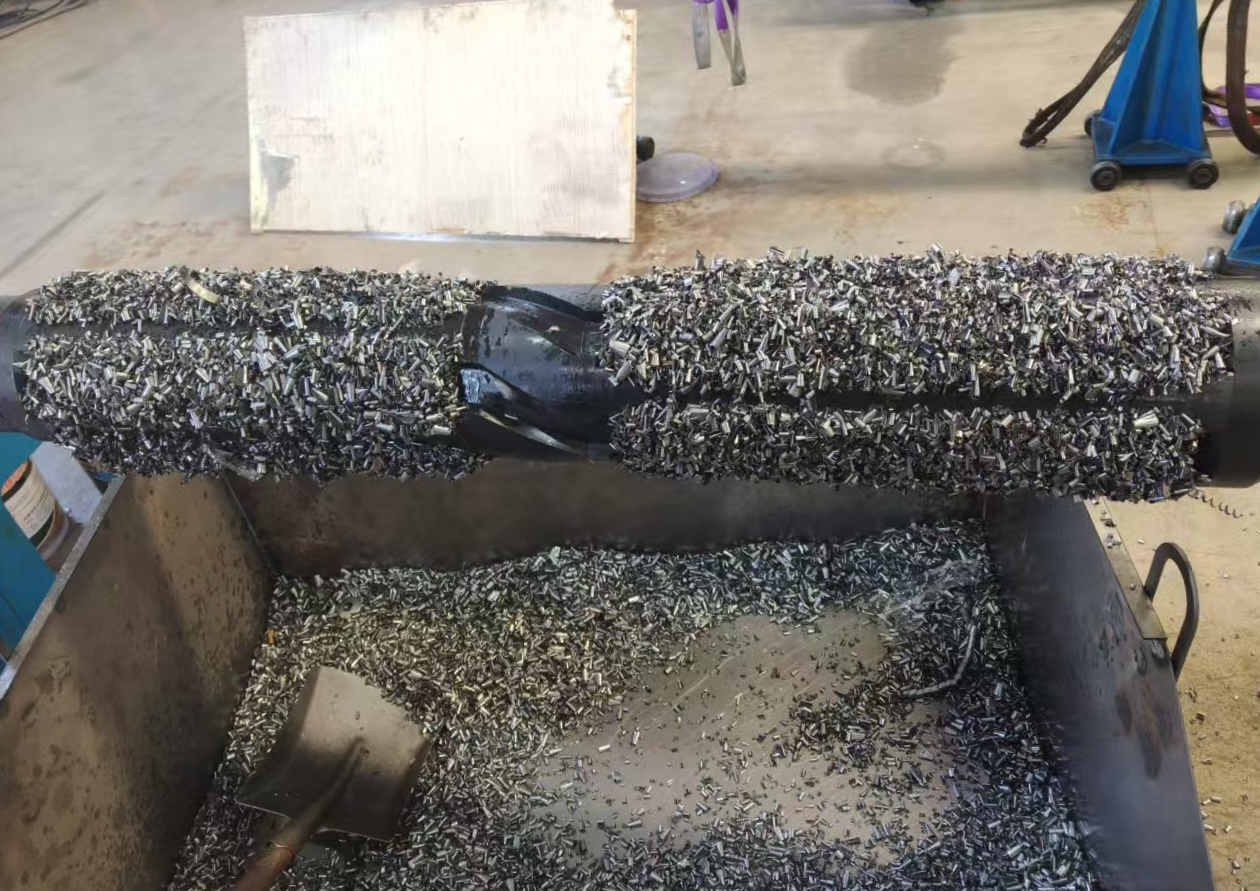
\includegraphics[width=0.6\textwidth]{figure/chapter3/magnetic-adsorption-capacity.jpg}
    \caption{大容量强磁工具吸附效果实测}
    \label{fig:magnetic_adsorption_capacity}
\end{figure}

\subsubsection{防退扣部分抗扭计算}
大容量强磁工具的防退扣主要薄点为下接头端面键（图纸DQC700007A--下接头）。下面为下接头端面键抗扭计算。端面键抗扭危险截面：为端面键截面（键的数量为6，图纸DQC700007A--下接头端面均布6条螺旋槽）。

防退扣抗扭强度 $\tau$ 计算：
\begin{equation}
    \begin{aligned}
        \tau &= \frac{T_{\max}}{3 \cdot b \cdot h \cdot d} \times 10^{-6} \\
        T_{\max} &= \frac{3 \cdot [\tau] \cdot b \cdot h \cdot d}{n_1} \times 10^{-6} \\
        [\tau] &= n \cdot \sigma_s = 0.66 \times 827\,\text{MPa} = 545.82\,\text{MPa}
    \end{aligned}
\end{equation}
式中，$T_{\max}$--最大防退扣扭矩，$\text{kN}\cdot\text{m}$（设计指标 $\ge 18$\,kN$\cdot$m，见本节脚注所列合同条款 5.2.1.3（2）：抗扭 $\ge 18\ \mathrm{kN} \cdot \mathrm{m}$）；

$\sigma_{\mathrm{s}}$--材料屈服应力，MPa（取 827\,MPa，按端面键材料 4145H 的屈服强度，见图号 DQC700007A--下接头技术要求第 1 条：调质后屈服强度 $\ge 827$\,MPa）；

$d$--端面键所在圆的直径，mm（取 73.5\,mm，图号 DQC700007A--下接头主视图标注的端面键分布圆直径）；

$b$--参与受剪的端面键宽度，mm（取 19\,mm，图号 DQC700007A--下接头端面键截面标注）；

$h$--端面键高度，mm（取 11.75\,mm，图号 DQC700007A--下接头端面键截面标注）；

系数3--按端面键靠侧面受剪、半周 3 个键参与传力的简化模型取值（若按端面键沿整个圆周均布、图号 DQC700007A--下接头端面均布的 6 条螺旋槽同时受剪计算，该系数应取 6）；

$n$--许用剪应力与许用拉应力系数，取 $n = 0.66$（按《机械设计手册》零件强度校核中许用应力折减系数的取值规定\cite{ref26}）；

$[\tau]$--材料许用切应力，MPa（按 $[\tau]=n\sigma_{\mathrm{s}} = 0.66\times 827$\,MPa 计算）；

$n_1$--安全系数，取 $n_1 = 1.5$（按《机械设计手册》机械零部件强度计算中安全系数的取值规定\cite{ref26}）。

下接头端面键截面防退扣最大扭矩：
\begin{equation}
    \begin{aligned}
        T_{\max} &= \frac{3 \cdot [\tau] \cdot b \cdot h \cdot d}{n_1} \times 10^{-6} \\
                 &= \frac{3 \times 545.82 \times 19 \times 11.75 \times 73.5}{1.5} \times 10^{-6} \\
                 &= 17.87\,\text{kN}\cdot\text{m}
    \end{aligned}
\end{equation}

需要说明的是，上述计算值为按半周3个端面键受剪、且计入安全系数$n_1 = 1.5$后的\textbf{许用}防退扣扭矩。该值略低于合同规定的抗扭$\ge 18\,\text{kN}\cdot\text{m}$设计指标，其原因是端面键为螺纹退扣的\textbf{后备}防退结构，而非工具的主传扭路径：工具的主传扭由心轴2.85\inch-8 Stub ACME螺纹承担（外螺纹根部35.98\,kN$\cdot$m、内螺纹根部86.29\,kN$\cdot$m，均远大于18\,kN$\cdot$m），端面键的作用是在扭矩与振动导致螺纹趋于退扣时才参与承载。若按6个端面键全部同时受剪计算，其许用防退扣扭矩为35.7\,kN$\cdot$m，可满足指标要求。


综合上述，强磁工具的强度参数见表\ref{tab:mag_tool_force_data}。

\begin{table}[htbp]
    \centering
    \caption{强磁工具受力件数据统计表}
    \label{tab:mag_tool_force_data}
    \renewcommand{\arraystretch}{1.5} % 增加行高，使表格更美观
    \begin{tabularx}{.9\textwidth}{CC}
        \toprule
        受力类型 & 数据 \\
        \midrule
        NC38 最大拉力 & $3000\,\text{kN}$ \\
        材料屈服强度 $\sigma_{\mathrm{s}}$ & $930\,\text{MPa}$ \\
        螺纹最大剪切力 $F_{\max1}$ & $2950.16\,\text{kN}$ \\
        心轴最大拉力 $F_{\max2}$ & $1627.42\,\text{kN}$ \\
        NC38 最大扭矩 & $41.30\,\text{kN}\cdot\text{m}$ \\
        材料许用切应力 $[\tau]$ & $620\,\text{MPa}$ \\
        心轴最大扭力 $T_{\max1}$ & $35.96\,\text{kN}\cdot\text{m}$ \\
        防退扣最大扭矩 $T_{\max2}$ & $17.87\,\text{kN}\cdot\text{m}$ \\
        \bottomrule
    \end{tabularx}
\end{table}


\subsection{永磁材料选型}
\label{citimoni}
高强磁性体是指那些能够产生强磁场，并在长时间内保持稳定磁性特性的材料。这些材料广泛应用于各种需要强磁力的工业和技术领域。高强磁性体的种类有很多，其中最常见的包括钕铁硼（NdFeB）、钐钴（SmCo）和铝镍钴（AlNiCo）等。在油井清洁打捞作业中，高强磁性体是大容量强磁工具的核心构件。
本项目将以井筒环境为应用基础，调研高强磁性体及高温磁性体的性能，对比筛选出最优产品，建立含磁工具关键结构的数值模拟模型，优化磁性体最大磁性布置规律、给出磁性体安放位置建议，结合磁性体消磁因素分析，给出最优的应用方式，提高工具使用寿命。本章的内容安排如下：

1) 调研钕铁硼、铝镍钴、钐钴等永磁材料在不同温度下的退磁曲线，调研材料退磁的影响因素，对比选择最优永磁材料；

2) 利用ANSYS Maxwell仿真平台建立强磁工具仿真模拟模型，通过改变永磁体充磁方向，探究磁体最大磁性布置规律；

3) 分别建立侧吸强磁结构和环吸强磁结构的仿真模型，探究两种结构对强磁工具最大磁性分布的影响；

4) 通过改变强磁工具上骨架的材料，研究骨架是否为导磁材料对强磁工具最大磁性的影响规律。


永磁材料选择时，应衡量材料工作温度，各温度下的内禀矫顽力（$H_\mathrm{cj}$）、各温度下的最大磁能积$(BH)_{\max}$等多因素。井筒清洁工具用永磁铁选型的主要依据是工作温度，本项目规定工具的温度设计指标是$150\,^\circ\mathrm{C}$。在满足使用温度的前提下，选择最大磁积能更大的永磁材料，这类次才具有更大的磁性。优先选择内禀矫顽力较大的材料，该类磁材的抗退磁能力和耐温性能更佳，可使得工具在复杂的井筒环境中的具有较好的磁性保持能力，赋予工具良好的稳定性和可靠性。此外还要考虑磁材的经济性和可获得性等辅助因素。

经调研发现，符合井筒清洁工具应用场景的可能材料如表\ref{tab:magnet_params}所示，两种典型磁材：烧结钐钴磁铁（SmCo5）和钕铁硼（N45UH）在不同温度下的退磁曲线如图\ref{fig:demagnetization_SmCo5}、\ref{fig:demagnatization_N45UH}所示。可知，SmCo5在$150\,^\circ\mathrm{C}$-$200\,^\circ\mathrm{C}$的高温环境下，其$H_\mathrm{cj}$在$14.2\sim 15.8\mathrm{kOe}$之间；N45UH永磁材料在$150\,^\circ\mathrm{C}\sim 200\,^\circ\mathrm{C}$的高温环境下，其$H_\mathrm{cj}$在$6.0\sim 9.0\mathrm{kOe}$之间。两数据对比可知，虽然在地面环境中N45UH的表观磁性更强，但是当工具下井后，温度升高，其磁性将大大衰减，于是其使用温度一般不超过$120\,^\circ\mathrm{C}$。SmCo5永磁材料因其$H_\mathrm{cj}$更高，其耐温性和抗退磁能力更好，考虑到本项目中清洁工具$150\,^\circ\mathrm{C}$的设计耐温指标，于是，选用钐钴材料为宜。

\begin{table}[htbp]
    \centering
    \caption{各类永磁材料的性能参数表}
    \label{tab:magnet_params}
    \begin{tabularx}{.9\textwidth}{CCC}
        \toprule % 顶部粗线
        材料类别 & 居里温度 & 最高工作温度 \\
        \midrule % 中间细线
        铝镍钴 AlNiCo & $750\sim 850^\circ\text{C}$ & $450\sim 550^\circ\text{C}$ \\
        铁氧体 Ferrite & $> 450^\circ\text{C}$ & $250^\circ\text{C}$ \\
        钐钴 SmCo5 & $700\sim 850^\circ\text{C}$ & $250\sim 350^\circ\text{C}$ \\
        钕铁硼 H系列 & $340^\circ\text{C}$ & $120^\circ\text{C}$ \\
        \bottomrule % 底部粗线
    \end{tabularx}
\end{table}

\begin{figure}[htbp]
	\centering
	\includegraphics[width=0.7\textwidth]{figure/chapter3/demagnetization-SmCo5.png}
	\caption{烧结钐钴磁铁（SmCo5）在不同温度下的退磁曲线}
	\label{fig:demagnetization_SmCo5}
\end{figure}

\begin{figure}[htbp]
	\centering
	\includegraphics[width=0.7\textwidth]{figure/chapter3/demagnatization-N45UH.png}
	\caption{钕铁硼（N45UH）磁铁在不同温度下的退磁曲线}
	\label{fig:demagnatization_N45UH}
\end{figure}

\subsection{井筒清洁工具中磁铁布置研究}
在井筒清洁工具中实现磁铁的安装，重点需要考虑的是磁铁部件的安转和夹紧，便于工具的使用和维护，这种结构设计工作甚至需要借鉴设计者在井下工具结构设计方面的经验。在确定工具的基本结构后，需要重点考察磁铁的磁化以其他辅助结构的选材等问题。图为本项目设计的大容量强磁工具，其主要的功能单元包含侧吸强磁和环吸强磁结构（如图2.3(b)、(c)）所示，两部分采用改了不同吸附结构，前者适于吸附小尺度铁质颗粒，后者适于吸附大尺度的铁质颗粒。侧吸强磁的磁铁放置于带窗的磁铁保护管中，增加与小尺度颗粒的接触面积，每个吸附单元包含两组磁铁，铁质碎屑将吸附于相邻吸附单元之间的空隙中。环吸强磁采用开放式结构，磁铁的外圆面暴露于外，增强对大尺寸的铁质碎屑的捕捉能力。给定磁铁材料和吸附结构的情况下，工具的吸附能力主要依赖于磁铁的磁化方向和结构件的材料，下文将对此展开仿真研究。



\subsubsection{强磁工具吸附力理论模型}
在井下环境中，强磁工具上永磁体对井筒内磁性碎屑的吸附主要源于永磁体所产生的磁场与磁性材料的相互作用，磁性碎屑在永磁体磁场中被磁化产生磁性并与永磁体产生相互作用力。此过程受磁场分布规律、磁场衰减特性、磁性材料磁化程度等多因素影响。
假设磁场均匀分布且磁性碎屑与强磁工具上的永磁体直接接触时，其吸附力可利用麦克斯韦应力公式计算：
\begin{equation}
	F=\frac{B^2A}{2\mu_0}
\end{equation}
式中，$B$--永磁体与磁性物质接触表面的磁感应强度，$\mathrm{T}$；

$A$--永磁体与磁性物质的接触面积，$\mathrm{m}^2$；

$\mu_0$--真空磁导率常数，$\mu_0=4\pi\times 10^{-7} \mathrm{H/m}$。

当磁性铁屑与磁铁存在一定距离$d$时，吸附力需考虑磁场梯度的影响，这时永磁体对磁性碎屑的吸引力可表示为
\begin{equation}
	F=\frac{3\mu_0 m_1m_2}{4\pi d^4}
\end{equation}
式中，$m_1$--永磁体的磁矩，A$\cdot$m$^2$；

$m_2$--磁性物质的磁矩，A$\cdot$m$^2$。

永磁体磁矩$m_1$的计算式为
\begin{equation}
	m_1=\frac{B_\mathrm{r}V_1}{\mu_0}
\end{equation}
式中，$B_\mathrm{r}$--永磁体剩磁，$\mathrm{T}$；

$V_1$--永磁体体积，$\mathrm{m}^3$。

铁屑的磁矩$m_2$与所处的外磁感应场强度$B$有关，计算式为
	\begin{equation}
		m_2 = \frac{\gamma B V_2}{\mu_0}
	\end{equation}
式中，$\gamma$--磁性物质的磁化率（量纲为 1，通常铁磁材料的 $\gamma \gg 1$）；

$V_2$--磁性物质体积，m$^3$。

综合以上两式，铁屑受到的磁力为
\begin{equation}
	F=\frac{3V_1V_2BB_r\gamma}{4\pi d^4}
\end{equation}

综上所述，在井下强磁工具吸附磁性碎屑过程中，当永磁体体积参数确定时，体积越大、距离工具越近，周围磁场强度更高的磁性碎屑所受吸附力越大。在井下碎屑参数未知时，可选择高温度下剩磁高、体积大的磁体，以及保证工具外侧磁场强度大来产生足够大的吸附力。但采用解析方法精确计算碎屑受到的磁力难度较大：一方面，单个永磁体要受到其他永磁体及工具复杂结构的影响，永磁体的剩磁$B_\mathrm{r}$难以确定；另一方面，磁性碎屑相互有之间会产生磁场的干扰，磁性碎屑堆积形成的碎屑床形状不规则，碎屑和磁铁之间的距离不能事先预测。于是，下文采用有限元的方法对工具空载（没有磁性碎屑存在）的条件下对工具周围磁场进行研究，作为一个表征工具碎屑吸附性能的间接指标，进而探索对工具性能产生影响的结构参数的影响。

\subsubsection{上部结构磁铁仿真模拟}

侧吸强磁结构为一三维结构，工具中的磁场应是一个复杂的三维空间磁场。但除端部外，其有效的功能单元是可看成是沿轴向均布的，于是，可考虑采用采用二维模型对所研究的问题进行简化。在ANSYS Maxwell软件中建立如图2.5所示的Maxwell 2D静磁场。永磁体材料选择井筒工作温度为$180\,^\circ \mathrm{C}$下的钐钴（SmCo5）材料，骨架材料选择4145牌号的钢材，永磁体保护套材料为304钢，各材料的属性列举于表\ref{tab:smco5_params}$\sim$表\ref{tab:304_properties_180c}中。


\begin{figure}[htbp]
	\centering
	\includegraphics[width=0.5\textwidth]{figure/chapter3/magnet-configuration-upper-sub.png}
	\caption{强磁工具上部结构模型}
	\label{fig:magnet_configuration_upper_sub}
\end{figure}



\begin{table}[htbp]
    \centering
    \caption{$180\,^\circ\mathrm{C}$ SmCo5磁材性能参数表}
    \label{tab:smco5_params}
    \begin{tabularx}{.9\textwidth}{CCCC}
        \toprule
        参数 & 符号 & 数值 & 单位 \\
        \midrule
        相对磁导率 & $\mu$ & 1.09 & -- \\
        剩磁 & $B_\mathrm{r}$ & 0.8 & T \\
        电导率 & $\sigma$ & 1500000 & Siemens/s \\
        %\midrule
        矫顽力 & $H_{\mathrm{cj}}$ & $15$ & kOe \\
        \bottomrule
    \end{tabularx}
\end{table}

\begin{table}[htbp]
    \centering
    \caption{$180\,^\circ\mathrm{C}$ 4145钢材性能参数表}
    \label{tab:steel_params}
    \begin{tabularx}{.9\textwidth}{CCCC}
        \toprule
        参数 & 符号 & 数值 & 单位 \\
        \midrule
        相对磁导率 & $\mu$ & 200 & -- \\
        电导率 & $\sigma$ & 4250000 & Siemens/s \\
        杨氏模量 & $E$ & 195 & GPa \\
        泊松比 & $\nu$ & 0.3 & -- \\
        \bottomrule
    \end{tabularx}
\end{table}

\begin{table}[htbp]
  \centering
  \caption{$180\,^\circ \mathrm{C}$下304不锈钢性能参数表}
  \label{tab:304_properties_180c}
  \begin{tabularx}{.9\textwidth}{CCCC}
    \toprule
    参数 & 符号 & 数值 & 单位 \\
    \midrule
    相对磁导率 & $\mu$ & 1 & -- \\
    电导率 & $\sigma$ & 1200000 & Siemens/s \\
    杨氏模量 & $E$ & 185 & GPa \\
    泊松比 & $v$ & 0.3 & -- \\
    \bottomrule
  \end{tabularx}
\end{table}


对于图\ref{fig:magnet_configuration_upper_sub}给定的磁铁、保护套和骨架结构，磁铁有图\ref{fig:two_magnetization_upper_sub}所示两种磁化方向，下文分别称为径向磁化和周向磁化。求解域设置为边长300mm的矩形，在其四条边上设置气球边界条件，网格划分，磁体与其保护套上最大网格尺寸0.5mm，上部结构骨架上最大网格尺寸2mm，求解步设置计算至收敛。在计算域中设置一个边长为200mm的矩形观测区域以观测仿真结果，以进行仿真结果后处理。

\begin{figure}[htbp]
    \centering
    % 子图 (a)
    \subfloat[径向磁化]{%
        \includegraphics[width=0.35\linewidth]{figure/chapter3/radial-magnetization-in-upper-sub.png}%
        \label{fig:radial_magnetization_in_upper_sub}
    }
    %\hfill
    % 子图 (b)
    \subfloat[周向磁化]{%
        \includegraphics[width=0.35\linewidth]{figure/chapter3/circumferencial-magnetization-in-upper-sub.png}%
        \label{fig:circumferencial_magnetization_in_upper_sub}%
    }
        \caption{侧吸强磁两种磁化方向示意图}
    \label{fig:two_magnetization_upper_sub}
\end{figure}

\begin{figure}[htbp]
    \centering
    % 子图 (a)
    \subfloat[边界条件设置]{%
        \includegraphics[width=0.35\linewidth]{figure/chapter3/boundary-condition-upper-sub.png}%
        \label{fig:boundary_condition_upper_sub}
    }
    %\hfill
    % 子图 (b)
    \subfloat[计算域网格划分]{%
        \includegraphics[width=0.35\linewidth]{figure/chapter3/mesh-upper-sub.png}%
        \label{fig:mesh_upper_sub}%
    }
        \caption{侧吸强磁磁场分析设置}
    \label{fig:computation_setup_upper_sub}
\end{figure}

(1) 径向充磁仿真结果及讨论

由于强磁工具在其使用工况下是通过其外侧磁场的作用吸附碎屑，因此在仿真结果中以强磁工具表面磁场强度为分析对象。

由观测面上的磁感应强度云图可知，最大磁感应强度出现在永磁体安装T型骨架沟槽的顶部和底部；各永磁体表面的$B$在$0.5\sim 1.5\mathrm{T}$范围内，但是受304不锈钢制的永磁体保护套影响，保护套外侧$B$在$0.2\sim 0.7\mathrm{T}$范围内，T型骨架表面的$B$在$0.6\sim 1.4\mathrm{T}$范围内，而圆形骨架的B较低大部分在$0.5\mathrm{T} $以下，从结果来看，304不锈钢制的永磁体保护套会使工具外侧的磁场强度变低。

\begin{figure}[htbp]
    \centering
    % 子图 (a)
    \subfloat[磁场矢量分布]{%
        \includegraphics[width=0.45\linewidth]{figure/chapter3/magnetic-vector-distribution-upper-sub.png}%
        \label{fig:magnetic_vector_distribution_upper_sub}
    }
    %\hfill
    % 子图 (b)
    \subfloat[磁感应强度分布]{%
        \includegraphics[width=0.45\linewidth]{figure/chapter3/contour-magnetic-field-upper-sub.png}%
        \label{fig:contour_magnetic_field_upper_sub}%
    }
        \caption{磁铁径向磁化时侧吸强磁组件磁场计算结果}
    \label{fig:field_result_in_upper_sub_radial_magnetization}
\end{figure}

(2) 周向充磁仿真结果及讨论

观察磁感应强度云图可知，观测面上最大磁感应强度$B=2.9\mathrm{T}$，出现在T型骨架沟槽最顶部，永磁体内的$B$在$0.6\sim 1.3\mathrm{T}$范围内，保护套上$B$在$0.5\sim 0.9\mathrm{T}$范围内，T型骨架沟槽中的B在$0.4\sim 1.3\mathrm{T}$范围内，而圆形骨架的$B$值在$0.3\sim 0.8\mathrm{T}$范围内。

\begin{figure}[htbp]
    \centering
    % 子图 (a)
    \subfloat[磁场矢量分布]{%
        \includegraphics[width=0.45\linewidth]{figure/chapter3/magnetic-vector-distribution-upper-sub-circum-magnatization.png}%
        \label{fig:magnetic_vector_distribution_upper_sub_circum_magnatization.png}
    }
    \hfill
    % 子图 (b)
    \subfloat[磁感应强度分布]{%
        \includegraphics[width=0.45\linewidth]{figure/chapter3/contour-magnetic-field-upper-sub-circum-magnatization.png}%
        \label{fig:contour_magnetic_field_upper_sub_circum_magnatization}%
    }
        \caption{磁铁周向磁化时侧吸强磁组件磁场计算结果}
    \label{fig:field_result_in_upper_sub_circum_magnetization}
\end{figure}


上部结构中的两种充磁方式中，周向充磁磁场分布更加均匀，但最大磁感应强度值远小于径向充磁磁场，分析得出上部结构类型导致T型骨架和圆形骨架上的磁场分布存在差异，T型骨架上的场强大于圆形骨架上场强，不锈钢制的磁铁保护套会降低永磁体表面的磁场强度。分析两种充磁方式下各部表面磁感应强度表可知，周向充磁与径向充磁相比，永磁体及其保护套、T形骨架表面上的磁场强度差异较小，但圆形骨架表面磁场强度大于周向充磁时的磁场强度，周向充磁时磁场分布更加均匀，因此，对于上部结构宜选用周向充磁方式。

%这里差一个表2.5

\subsubsection{下部结构仿真模拟}

强磁工具下部结构为一对称结构，永磁体均匀排列在其骨架上，为方便仿真计算，将下部结构简化为二维模型求解，在ANSYS Maxwell软件中建立如图\ref{fig:magnet_configuration_lowwer_sub}所示的强磁工具下部结构仿真模型。永磁体材料选择井筒工作温度为180℃下的钐钴SmCo5材料，骨架材料选择4145牌号的钢材，各材料的属性见表\ref{tab:smco5_params}$\sim$表\ref{tab:304_properties_180c}。

\begin{figure}[htbp]
	\centering
	\includegraphics[width=0.5\textwidth]{figure/chapter3/magnet-configuration-lowwer-sub.png}
	\caption{强磁工具上部结构模型}
	\label{fig:magnet_configuration_lowwer_sub}
\end{figure}

对于强磁工具下部结构，磁铁有图2.6所示的同一径向磁化、交叉径向磁化、周向磁化三种磁化方向，其他仿真参数与上部结构仿真模型相同，如图\ref{fig:computation_setup_lowwer_sub}所示，对观测面上的仿真结果进行分析。三种磁化方式对应的磁场分布如图\ref{fig:field_result_in_lowwer_sub_3_magnetization}所示。


\begin{figure}[htbp]
    \centering
    % 子图 (a)
    \subfloat[同一径向磁化]{%
        \includegraphics[width=0.4\linewidth]{figure/chapter3/lowwer-sub-magnetization-radial.png}%
        \label{fig:lowwe_sub_magnetization_radial}%
    }
    \vspace{1em}
    % 子图 (b)
    \subfloat[交叉径向磁化]{%
        \includegraphics[width=0.4\linewidth]{figure/chapter3/lowwer-sub-cross-magnetization.png}%
        \label{fig:lowwer_sub_cross_magnetization}
    }
    \hfill
    % 子图 (c)
    \subfloat[周向磁化]{%
        \includegraphics[width=0.4\linewidth]{figure/chapter3/lowwer-sub-circumferential-magnetization.png}%
        \label{fig:lowwer_sub_circumferential_magnetization}%
    }
        \caption{环吸强磁磁化方向示意图}
    \label{fig:lowwer_sub_magnetization_3ways}
\end{figure}


\begin{figure}[htbp]
    \centering
    % 子图 (a)
    \subfloat[边界条件设置]{%
        \includegraphics[width=0.4\linewidth]{figure/chapter3/boundary-condition-lowwer-sub.png}%
        \label{fig:boundary_condition_lowwer_sub}
    }
    %\hfill
    % 子图 (b)
    \subfloat[计算域网格划分]{%
        \includegraphics[width=0.4\linewidth]{figure/chapter3/mesh-upper-sub.png}%
        \label{fig:mesh_lowwer_sub}%
    }
        \caption{环吸强磁磁场分析设置}
    \label{fig:computation_setup_lowwer_sub}
\end{figure}



\begin{figure}[htbp]
    \centering
    % 子图 (a)
    \subfloat[磁场矢量分布]{%
        \includegraphics[width=0.45\linewidth]{figure/chapter3/magnetic-vector-distribution-lowwer-sub-radial.png}%
        \label{fig:magnetic_vector_distribution_lowwer_sub_radial}
    }
    %\hfill
    % 子图 (b)
    \subfloat[磁感应强度分布]{%
        \includegraphics[width=0.45\linewidth]{figure/chapter3/contour-magnetic-field-lowwer-sub-radial.png}%
        \label{fig:contour_magnetic_field_lowwer_sub_radial}%
    }
    \vspace{1em}
     % 子图 (c)
    \subfloat[磁场矢量分布]{%
        \includegraphics[width=0.45\linewidth]{figure/chapter3/magnetic-vector-distribution-lowwer-sub-cross.png}%
        \label{fig:magnetic_vector_distribution_lowwer_sub_cross}
    }
   % \hfill
    % 子图 (d)
    \subfloat[磁感应强度分布]{%
        \includegraphics[width=0.45\linewidth]{figure/chapter3/contour-magnetic-field-lowwer-sub-cross.png}%
        \label{fig:contour_magnetic_field_lowwer_sub_cross}%
    }
    \vspace{1em}
     % 子图 (e)
    \subfloat[磁场矢量分布]{%
        \includegraphics[width=0.45\linewidth]{figure/chapter3/magnetic-vector-distribution-lowwer-sub-circumferential.png}%
        \label{fig:magnetic_vector_distribution_upper_sub_circumferential}
    }
   % \hfill
    % 子图 (f)
    \subfloat[磁感应强度分布]{%
        \includegraphics[width=0.45\linewidth]{figure/chapter3/contour-magnetic-field-lowwer-sub-circumferential.png}%
        \label{fig:contour_magnetic_field_upper_sub_circumferential}%
    }


        \caption{磁铁采用不同磁化方式时环吸强磁组件磁场计算结果}
    \label{fig:field_result_in_lowwer_sub_3_magnetization}
\end{figure}




(1) 同一径向充磁仿真结果及讨论

由观测面上的磁感应强度云图可知，磁感应强度成对称分布，最大磁感应强度$B=5.7 \mathrm{T}$，出现在永磁体安装骨架的肩槽和骨架沟槽顶部，各永磁体表面的$B$在$0.5\sim 1.5\mathrm{T}$范围内，骨架沟槽表面的$B$在骨架最凹处最小沿沟槽向两侧增大其数值在$0.5\sim 3.5\mathrm{T}$范围内。

(2) 交叉径向充磁仿真结果及讨论

由观测面上的磁感应强度云图可知，磁感应强度称对称分布，最大磁感应强度$B=3.8 \mathrm{T}$，出现在永磁体安装骨架的肩槽和骨架沟槽顶部，各永磁体表面$B$在$0.7\sim 1.5\mathrm{T}$范围内，骨架沟槽表面的$B$在$1.2\sim 3.5\mathrm{T}$范围内。

(3) 周向充磁仿真结果及讨论

由观测面上的磁感应强度云图可知，云图上最大磁感应强度出现在骨架沟槽最凹点处，各永磁体上的$B$在$1.3\sim 1.7\mathrm{T}$范围内，骨架沟槽表面最凹点$B$最大沿沟槽向两侧减小，其数值在$0.7\sim 3.5\mathrm{T}$范围内。


由基于充磁方式的环吸强磁工具仿真结果总结于表\ref{tab:magnetic_intensity}，由此可得出，永磁体表面的磁感应强度周向充磁时略强于径向充磁时，分析骨架沟槽的表面的磁感应强度可知，同一径向充磁和周向充磁时，骨架沟槽上的磁感应强度梯度大，交叉径向充磁时骨架沟槽表面的磁感应强度分布更均匀。同一径向充磁和周向充磁时，磁感线会富集到骨架沟槽内造成骨架沟槽内的磁感应强度大，而工具外侧的磁感应强度小。因此，下部结构宜选择交叉径向充磁方式。

\begin{table}[htbp]
    \centering
    \caption{下部结构各部表面磁感应强度数据}
    \label{tab:magnetic_intensity}
    \begin{tabularx}{.9\textwidth}{CCCC} % 第一列左对齐(l)，后三列居中(c)
        \toprule
        % 第一行：左侧标题 + 右侧跨3列的标题
        强磁工具结构 & \multicolumn{3}{c}{下部结构} \\
        \midrule
        % 第二行：具体的充磁类型分类
        充磁类型 & 同向径向充磁 & 交叉径向充磁 & 周向充磁 \\
        \midrule
        % 第三行：数据
        永磁体表面 & $0.5\sim 1.5\mathrm{T}$ & $0.7\sim 1.5\mathrm{T}$ & $1.3\sim 1.7\mathrm{T}$ \\
        % 第四行：数据
        骨架沟槽表面 & $0.5\sim 3.5\mathrm{T}$ & $1.2\sim 3.5\mathrm{T}$ & $0.7\sim 3.5\mathrm{T}$ \\
        \bottomrule
    \end{tabularx}
\end{table}

\subsection{两种结构对强磁工具最大磁性分布的影响}

本节依据上节两种强磁工具结构的仿真结果，通过数据对比分析两种结构对强磁工具磁性分布的影响。强磁工具各部表面磁感应强度数值由磁场探针测得，测量数据见表\ref{tab:strong_magnet_data}。



\begin{table}[htbp]
    \centering
    \caption{强磁工具各部表面磁感应强度数据表}
    \label{tab:strong_magnet_data}
    % 设置列格式：第一列左对齐，其余居中。p{}用于控制长文本换行
    \begin{tabular}{lcccccc}
        \toprule
        % 第一行表头：上部结构(跨2列)，下部结构(跨3列)
        强磁工具结构 & \multicolumn{2}{c}{上部结构} & \multicolumn{4}{c}{下部结构} \\
        \cmidrule(r){2-3} \cmidrule(l){4-7} % 子表头下方的横线，r/l控制留白
        % 第二行表头：具体的充磁类型
        充磁类型 & 径向充磁 & 周向充磁 & \shortstack{同向径向\\充磁} & \shortstack{交叉径向\\充磁} & \multicolumn{2}{c}{周向充磁} \\
        \midrule
        % 数据行 1
        永磁体表面 & $0.5\sim 1.5\mathrm{T}$ & $0.6\sim 1.3\mathrm{T}$ & $0.5\sim 1.5\mathrm{T}$ & $0.7\sim 1.5\mathrm{T}$ & \multicolumn{2}{c}{$1.3\sim 1.7\mathrm{T}$} \\
        % 数据行 2 (包含合并行 "骨架沟槽表面")
        T型骨架表面 & $0.6\sim 1.4\mathrm{T}$ & $0.4\sim 1.3\mathrm{T}$ & \multirow{2}{*}{\shortstack{骨架沟槽\\表面}} & $0.5\sim 3.5\mathrm{T}$ & $1.2\sim 3.5\mathrm{T}$ & $0.7\sim 3.5\mathrm{T}$ \\
        % 数据行 3
        圆形骨架表面 & $0\sim 0.3\mathrm{T}$ & $0.3\sim 0.8\mathrm{T}$ & & -- & -- & -- \\
        % 数据行 4
        保护套表面 & $0.2\sim 0.7\mathrm{T}$ & $0.5\sim 0.9\mathrm{T}$ & -- & -- & -- & -- \\
        \bottomrule
    \end{tabular}
\end{table}

由强磁工具的上、下部结构在不同充磁方向下的各部位表面磁场数据得出，对于上部结构，由于其结构影响T型骨架和圆形骨架上的磁场分布差异较大，T型骨架上场强大于圆形骨架上的场强，且不锈钢保护套会造成永磁体表面磁场衰减，改变永磁体充磁方向后磁场分布仍呈现此情况；对于下部结构，不同的充磁方向对其表面磁场分布影响很大，永磁体采用交叉径向充磁时，工具永磁体和骨架的表面磁场分布均匀。综上所述，采用交叉径向充磁的环吸强磁工具结构的表面磁场分布均匀，易于强磁工具在井筒内的大面积吸附工作。


\subsection{强磁工具骨架材料对最大磁性分布的影响}

利用2.2.4小节中的下部工具结构仿真模型数据，保持其他仿真参数不变，在永磁体交叉径向充磁的工况下，将强磁工具骨架材料设置为不导磁的铝材，铝材参数如表\ref{tab:aluminum_params}所示，观察仿真结果中工具表面磁场分布。下部结构交叉径向充磁时，铝制骨架与4145钢制骨架模型的仿真结果进行对比分析图\ref{fig:mag_field_frame_material}。

\begin{table}[htbp]
    \centering
    \caption{180$^\circ$C下铝材参数表}
    \label{tab:aluminum_params}
    \begin{tabularx}{.9\textwidth}{CCCC}
        \toprule
        参数 & 符号 & 数值 & 单位 \\
        \midrule
        相对磁导率 & $\mu$ & 1.00021 & -- \\
        电导率 & $\sigma$ & 38000000 & Siemens/s \\
        杨氏模量 & $E$ & 69 & GPa \\
        泊松比 & $\nu$ & 0.31 & -- \\
        \bottomrule
    \end{tabularx}
\end{table}

\begin{figure}[htbp]
    \centering
    % 子图 (a)
    \subfloat[4145钢制骨架]{%
        \includegraphics[width=0.4\linewidth]{figure/chapter3/mag-field-distribution-4145-steel-frame.png}%
        \label{fig:mag_field_distribution_4145_steel_frame}
    }
    \hfill
    % 子图 (b)
    \subfloat[铝制骨架]{%
        \includegraphics[width=0.4\linewidth]{figure/chapter3/mag-field-distribution-aliminium-frame.png}%
        \label{fig:mag_field_distribution_aliminium_frame}%
    }
        \caption{骨架材料对磁场分布的影响}
    \label{fig:mag_field_frame_material}
\end{figure}

表\ref{tab:aluminum_vs_4145_steel}为环吸强磁工具结构交叉径向充磁模型的4145钢制骨架和铝制骨架仿真结果对比。由铝制骨架仿真结果得出，铝制骨架导致工具磁场中的最大场强降低，铝制骨架沟槽内的磁场强度低于4145钢制骨架沟槽内的磁场强度，分析得出骨架材料宜选用导磁效果好，可磁化程度高的金属合金材料，以起到聚集磁感线增大磁通的效果。


\begin{table}[htbp]
    \centering
    \caption{铝制骨架与4145钢制骨架工具表面磁场数据对比}
    \label{tab:aluminum_vs_4145_steel}
    \begin{tabularx}{.9\textwidth}{CCC}
        \toprule
        强磁工具结构 & \multicolumn{2}{c}{下部结构} \\
        \cmidrule(r){2-3}
        充磁类型 & \multicolumn{2}{c}{周向充磁} \\
        \cmidrule(r){2-3}
        骨架材料 & 4145 钢制 & 铝制 \\
        \midrule
        永磁体表面 & $0.7\sim 1.5\mathrm{T}$ & $0.3\sim 0.7\mathrm{T}$ \\
        骨架沟槽表面 & $1.2\sim 3.5\mathrm{T}$ & $0.2\sim 0.4\mathrm{T}$ \\
        \bottomrule
    \end{tabularx}
\end{table}

\subsection{永磁材料的退磁影响因素}

永磁体的退磁是影响其长期稳定性和应用可靠性的关键问题，退磁由多种因素引起。

（1）居里温度

居里温度是磁性材料在铁磁性物质/亚铁磁性物质和顺磁性物质之间改变的温度。温度超过居里温度，磁体内部分子剧烈运动并出现不可逆的退磁情况，磁体退磁后可再次被充磁，但磁力会大幅下降，仅能达到原来的50\%左右。

（2）工作温度

在工作温度内温度升高磁力会下降，但是不超过居里温度的情况下，降温后磁力大部分会恢复，工作温度范围内发生可逆性退磁。

（3）外部磁场

外部强反向磁场（如电机电枢反应、短路电流）可能超过磁体的矫顽力，导致磁体部分或完全退磁。

（4）时间因素

随着时间的延长磁体内部微观结构（如晶粒边界、杂质相）随时间缓慢变化，导致剩磁轻微衰减，通常每年衰减小于1\%。

（5）机械冲击

机械应力可能破坏磁体内部的磁畴排列，尤其是脆性材料（如钕铁硼），避免直接敲击或跌落磁体。在复杂振动环境中增加缓冲结构（如橡胶垫）。

（6）化学侵蚀

在高温、高湿的酸碱环境下，钕铁硼磁体因含钕、铁易氧化（生锈），导致磁通量下降甚至断裂。在不稳定的化学环境下对磁体进行表面涂层（如镍、锌、环氧树脂、电镀层）或密封封装以隔绝环境影响。

具体到井筒清洁工具设计，具体到井筒清洁工具的设计，选择的钐钴磁铁耐温达到了$450\sim 550^\circ$C，磁材的居里温度为$750\sim 850^\circ$C，远超工具的设计温度指标150$^\circ$C，可保证磁铁不会因温度因素而退磁，在重复使用过程中，可保证磁材都是可逆退磁。井筒中不存在可能使磁铁退磁强外部磁场，磁铁在工作过程中的退磁效应可忽略。在工具长时间存储时，可考虑采用铁磁质材料制作的磁路附件使得磁材的磁路闭合，减少磁材磁性的衰减。在机械结构设计上，磁铁外设计了不锈钢制作的保护套，以减少清洁工具在运输和使用过程中产生的冲击直接作用于磁铁本身，减少机械冲击。在磁铁在制造过程中表面采用镀镍工艺，易蚀性磁材本体和腐蚀性的环境隔离开来，磁铁在安装过程中设置了安装规范，减少磁材表面划伤，严禁损伤磁材下井。

\subsubsection{强磁工具操作方式}

（1）使用方法

根据井眼尺寸选择合适的强磁吸附工具。强磁工具通过钻柱送入井底完成吸附打捞作业，如情况允许也可以通过钢丝绳送入井底。

（2）操作方法

该工具可以与模块化多合一套管清洁工具一同使用（推荐），也可以在刮完井之后使用。将强磁吸附工具放在预先放好木板的转盘上（防止强磁吸附工具与转盘发生吸附），并接于钻柱底部，然后提起，取掉木板，准备下井。将大容量强磁吸附工具下到井下离通井位置$3\sim 5\mathrm{m}$处，开泵循环。将大容量强磁吸附工具在该位置上下活动。保持循环，平稳地上提钻柱。起钻时要求平稳、低速、严禁剧烈震动与撞击，以保护强磁部件。

\subsubsection{强磁工具维护与保养}

大容量强磁吸附工具每次使用后，应放在没有铁屑和杂物区域内的木板或橡胶板上，清除干净吸附在强磁工具表面的金属颗粒和铁屑粉末，然后用清水清洗各零件。工具在井下工作多次后，或在恶劣条件下工作后，应进行维护修理，将其全部拆开、检查、重新装配。

\subsubsection{强磁工具检验与测试}

为确保强磁组件具有$150^{\circ}\mathrm{C}$的耐温标准，需对磁铁材料和整个强磁组件进行测试。磁铁材料的耐温性能需依据国家标准（GB/T 13560-2017）进行不可逆磁通损失检测。使用长径比（$L/D$）为$0.7$的标准圆柱体样品，在饱和磁化后，置于开路状态下加热至$150^{\circ}\mathrm{C}$并保温2小时，随后冷却至室温，测量值冷却后的开路磁通。若不可逆磁通损失应小于5\%，则说明该磁铁材料在$150^{\circ}\mathrm{C}$下耐温合格。

对于强磁组件，应进行高温烘烤测试。将组装好的磁铁或产品直接放入恒温烤箱中，在有$150^{\circ}\mathrm{C}$下保温2小时。取出冷却至室温后，测量其表磁或磁通量，对比加热前后的衰减比例应小于5\%。

为保证磁铁对紧贴表面的铁屑（材料以45钢为例）产生 $8 \mathrm{kg/cm²}$ 以上的吸附力\footnote{响应合同内容：5.2.1.3井筒高效清洁关键技术配套工具设计--大容量强磁吸附工具：吸附力$\ge 8 \mathrm{kg/cm²}$}，强磁工具在出厂时应使用磁强计对磁铁表面磁场进行测量，磁铁表面的磁感应强度需要达到 $0.4  \mathrm{T}$以上。测量前应清洁磁铁表面，确保磁铁表面平整，无铁屑残留，磁强计探头表面应紧贴磁铁表面，二者之间无间隙。

磁吸力的直接测定方法可参照国家标准 GB/T 47662-2026《磁性材料磁吸力测试方法》\footnote{GB/T 47662-2026，2026-07-02 发布，2027-02-01 实施；中国标准分类号（CCS）K14，国际标准分类号（ICS）29.030，归口部门为中国电器工业协会，发布单位为国家市场监督管理总局、国家标准化管理委员会。本文编制时该标准已发布、尚未实施。}执行。该标准规定了磁性材料磁吸力的测试方法，适用于磁性材料磁吸力的测定，可作为强磁工具出厂检验与型式试验中吸附力指标考核的方法依据。本报告编制时该标准已发布但尚未实施，故现场检验按参照执行的方式引用，待其正式实施后按其现行有效版本执行。

井下实际吸附对象为形状不规则、堆积状态随机的铁屑，其与磁体表面的贴合面积和间隙难以在检验中复现，直接测定吸附力时宜按上述标准以规定形状与材质的导磁试件（如45钢试片）替代铁屑，并记录试件材质、表面状态、贴合间隙与测试温度等条件，以保证测量结果的可复现性。在试件与磁体表面紧密贴合的极限条件下，吸附力 $F$、磁体表面磁感应强度 $B$ 与接触面积 $A$ 之间满足麦克斯韦应力关系 $F/A=B^{2}/(2\mu_0)$；要求吸附力不小于 $8\,\mathrm{kg/cm^2}$ 时，对应的磁感应强度为 $1.42\,\mathrm{T}$，与前述出厂磁强计检验的判据一致。因此，在不具备直接拉力试验条件时，可沿用磁强计测量磁体表面磁感应强度作为吸附力的间接表征；具备条件时宜按 GB/T 47662-2026 直接测定吸附力，并以两者互为验证。


\subsection{强磁工具适用井况、管柱组合与施工工艺}

\subsubsection{强磁工具适用井况}

强磁工具主要适用于以下井况：

\begin{itemize}
	\item 磨铣/射孔/大修后（井筒内产生大量铁屑）：套磨铣、开窗、侧钻、射孔、锻铣、切割后产生大量细$\sim$中粒铁屑，粒径从毫米级到厘米级，其特点是数量多、分散、循环难带出；
	\item 水平井/大斜度井（井斜$> 30^\circ$）：岩屑床与铁屑混合，低返速、携砂难、重力堆积；
	\item 低压/低返排/漏失井：地层压力低、循环漏失、液流携屑能力弱；
	\item 完井/关键工具下入前（净化保障）：下入封隔器、筛管等井下工具前清除铁屑，防止卡钻及刺穿、损坏密封件。
\end{itemize}

\subsubsection{强磁工具管柱组合}

强磁工具可根据作业目的与其它清洁工具组合使用，管柱组合（自下至上）如下：

（1）完井/关键工具下入前，清洁管壁：刮管器 $+$ 短钻杆 $+$ 大容量强磁吸附工具 $+$ 短钻杆 $+$ 震击器 $+$ 钻杆；

（2）套磨铣作业，大修打捞：套铣鞋/磨铣鞋 $+$ 短钻杆 $+$ 大容量强磁吸附工具 $+$ 短钻杆 $+$ 震击器 $+$ 钻杆；

（3）冲砂通井，小件落物打捞：冲砂工具/打捞工具 $+$ 短钻杆 $+$ 大容量强磁吸附工具 $+$ 短钻杆 $+$ 震击器 $+$ 钻杆。

\subsubsection{强磁工具施工工艺步骤}

强磁工具的现场施工按下列步骤进行：

（1）施工前准备；

（2）下钻作业：平稳下入管柱，控制下放速度，遇阻时严禁猛顿，下至设计深度时记录上提、下放悬重与空转扭矩；

（3）清洁作业；

（4）起钻作业；

（5）工具出井后清理与复检；

（6）注意事项：作业过程中应保持循环畅通，起钻平稳、低速，严禁剧烈震动与撞击，具体要求见前述强磁工具操作方式与维护保养的相关内容。




本节首先调研了钕铁硼、铝镍钴、钐钴等永磁材料的工作参数及退磁曲线，确定了钐钴材料为井下强磁工具上的永磁体材料并分析了永磁体退磁影响因素；其次，利用ANSYS Maxwell软件构建了侧吸强磁结构和环吸强磁结构的仿真模型，通过改变工具中永磁体充磁方式及骨架材料，探究其最大磁性分布规律；在基于充磁方向的磁体布置研究中得出，上部结构宜采用径向充磁方式，下部结构宜采用周向充磁方式来达到磁场分布均匀且保证最大磁性的目的；在基于骨架材料对最大磁性分布的影响研究中得出，骨架材料为导磁效果好的金属材料时，能聚集磁感线增大磁通，起到增加工具磁性的作用。




























































